 \chapter{Methodology}\label{ch:methodology}

\section{Introduction}\label{sec:intro}

In this chapter, the development process for \textbf{Collective} mobile journaling application is explained using the Rapid Application Development (RAD) methodology. Each stage of the developemnt is explained in detail, covering the phases of requirements planning, user design, construction and cutover.

\section{Rapid Application Development (RAD) Methodology}\label{sec:rad}

\begin{figure}[H]
\centering
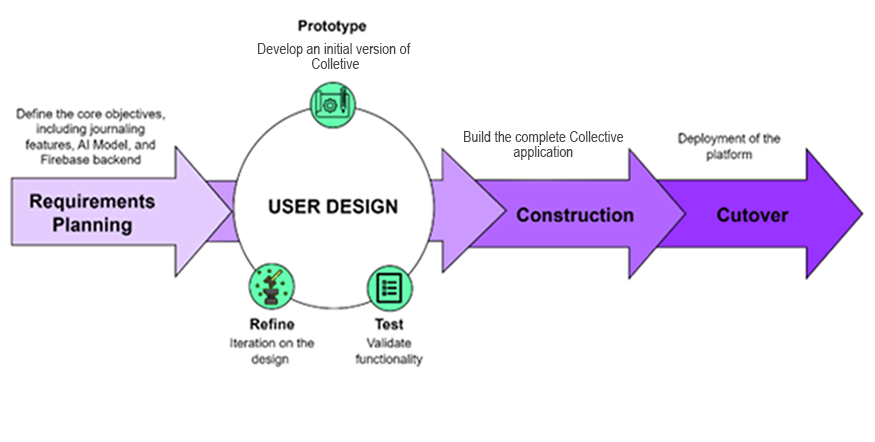
\includegraphics[width=0.8\textwidth]{files/imgs/RAD.png}
\caption{Rapid Application Development (RAD) Methodology Phases}
\label{fig:rad-methodology}
\end{figure}

Rapid Application Development (RAD) is a software development methodology that emphasizes quick development and iteration of prototypes over rigorous planning and testing. It is particularly useful for projects where requirements are expected to evolve or are not fully understood at the outset. The RAD methodology consists of four main phases: requirement planning, user design, construction, and cutover. This model was chosen for the development of the \textbf{Collective} mobile journaling application due to its flexibility and focus on user feedback, which is crucial for creating a user-friendly and effective application. The detais of the project is discussed below:

\section{Requirement planning}\label{sec:requirementPlanning}   

The requirement planning phase is the first step in the RAD methodology, where the project team identifies and defines the requirements of the application. This phase involves gathering information from stakeholders, including potential users, to understand their needs and expectations. The goal is to create a clear and concise set of requirements that will guide the development process.

\subsection{Software Requirements}\label{subsec:softwareRequirements}

The following tables list the sofware and tools used to develop the \textbf{Collective} mobile journaling application:

\subsection{Hardware Requirements}\label{subsec:hardwareRequirements}
\subsection{Use Case Diagram}\label{subsec:usecaseDiagram}
\subsection{Use Case Description}\label{subsec:usecaseDescription}

\section{User design}\label{sec:userDesign}